\documentclass[conference]{IEEEtran}
\usepackage{graphicx}
\usepackage{amsmath}
\usepackage{cite}
\usepackage{tikz}
\usetikzlibrary{arrows.meta,positioning,fit,backgrounds,angles,quotes,calc}

\begin{document}

\title{ARGUS: Real-Time Perception-Aware MPC for Aerial Target Tracking with ESDF Obstacle Avoidance}

\author{\IEEEauthorblockN{Bruno Pinto}}

\maketitle

\begin{abstract}
This paper extends a perception-aware model predictive controller for aerial target tracking. The controller was originally implemented in Python, with CasADi and IPOPT as the solver and obstacles represented as known analytical shapes \cite{pinto_thesis}. It is ported here to C++, solved in real time with acados, with obstacles now represented by a Euclidean signed distance field (ESDF) built from simulated onboard sensing instead of known shapes. Two further extensions are added on top of this port: collision avoidance is moved from a soft cost term to a slacked nonlinear constraint, and an occlusion-aware cost term is introduced to penalize obstacles blocking the line of sight to the target. The main contribution is a derivation showing that the occlusion cost, in its natural point-linearization form, has a gradient that structurally vanishes as the occluding obstacle approaches the target, independent of cost weight. Two candidate fixes, hard-min versus soft-min aggregation of multiple fixed sightline samples, and a steeper penalty function, are derived and tested, and both are shown to leave the underlying vanishing-gradient problem untouched. The root cause is identified as a geometric property of the point-interpolation parametrization itself, not a tuning or sampling artifact, pointing toward an angular or frustum-based formulation as the direction with different sensitivity near the target.
\end{abstract}

\begin{IEEEkeywords}
Trajectory Optimization, Model Predictive Control, Occlusion Avoidance, Aerial Target Tracking, Perception-Aware Planning
\end{IEEEkeywords}

\section{Introduction}

Autonomous aerial tracking of a moving target through cluttered environments requires a controller that keeps the target in view, avoids collisions, and produces a trajectory the vehicle can actually fly. A first version of this controller was built in Python \cite{pinto_thesis}, using CasADi and IPOPT as the solver, with obstacles represented as known analytical shapes rather than sensed online.

This paper reports on three extensions made since. First, I ported the controller to C++, solved in real time with acados \cite{acados}, and replaced the known analytical obstacle shapes with an ESDF built from simulated onboard sensing. Second, collision avoidance is moved from a soft cost term to a slacked nonlinear constraint. Third, an occlusion-aware cost term, absent from the original formulation, is added to penalize obstacles blocking the line of sight to the target. The first two extensions are reported briefly. The third is the main subject of the paper: the occlusion cost is derived, its gradient is shown to vanish structurally in a specific, common geometric case, and two plausible fixes are tested and shown not to resolve it. Section~\ref{sec:future} states plainly what remains open.

\section{System Architecture}
\label{sec:arch}

\begin{figure}[t]
\centering
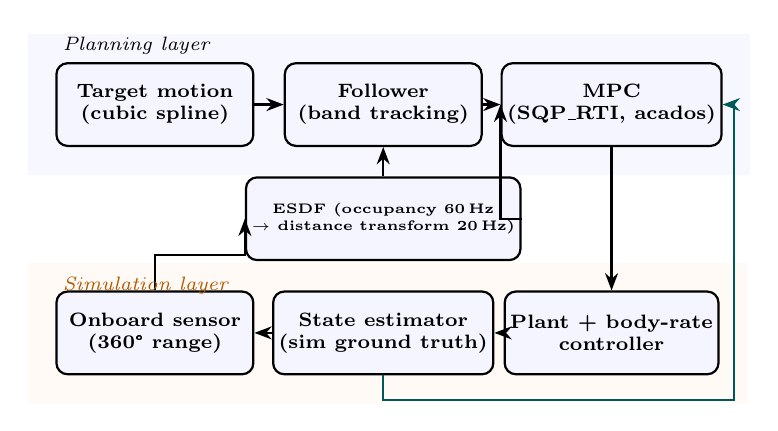
\begin{tikzpicture}[
  box/.style={draw, rounded corners, fill=blue!4, minimum width=2.5cm, minimum height=1.05cm,
              align=center, font=\scriptsize\bfseries, inner sep=2pt},
  >={Stealth[length=2.2mm]}, thick
]
\node[box] (target) at (0,3.3) {Target motion\\(cubic spline)};
\node[box] (follower) at (2.9,3.3) {Follower\\(band tracking)};
\node[box] (mpc) at (5.8,3.3) {MPC\\(SQP\_RTI, acados)};

\node[box, minimum width=3.1cm, font=\tiny\bfseries] (esdf) at (2.9,1.85)
  {ESDF (occupancy 60\,Hz\\$\rightarrow$ distance transform 20\,Hz)};

\node[box] (sensor) at (0,0.4) {Onboard sensor\\(360\textdegree\ range)};
\node[box] (state) at (2.9,0.4) {State estimator\\(sim ground truth)};
\node[box] (plant) at (5.8,0.4) {Plant + body-rate\\controller};

\begin{scope}[on background layer]
\node[fill=blue!3, fit=(target)(follower)(mpc), inner sep=10pt] {};
\node[fill=orange!4, fit=(sensor)(state)(plant), inner sep=10pt] {};
\end{scope}

\coordinate (p1) at (2.9,-0.45);
\coordinate (p2) at (7.35,-0.45);
\coordinate (p3) at (7.35,3.3);

\draw[->] (target.east) -- (follower.west);
\draw[->] (follower.east) -- (mpc.west);
\draw[->] (esdf.north) -- (follower.south);
\draw[->] (esdf.east) -| (mpc.west);
\draw[->] (sensor.north) -- ++(0,0.45) -| (esdf.west);
\draw[->] (state.west) -- (sensor.east);
\draw[->] (plant.west) -- (state.east);
\draw[->] (mpc.south) -- (plant.north);
\draw[->, color=teal!70!black] (state.south) -- (p1) -- (p2) -- (p3) -- (mpc.east);

\node[font=\scriptsize\itshape, anchor=west] at (-1.3,4.05) {Planning layer};
\node[font=\scriptsize\itshape, anchor=west, color=orange!70!black] at (-1.3,1.0) {Simulation layer};
\end{tikzpicture}
\caption{System architecture. Binary occupancy is rebuilt every sensor sweep (60 Hz); the ESDF is rebuilt once per control tick (20 Hz). The teal path is the state-feedback loop closing the control loop back into the MPC.}
\label{fig:architecture}
\end{figure}

The system is implemented in C++, generating the MPC solver through acados \cite{acados} from a symbolic CasADi model (Fig.~\ref{fig:architecture}). The target's trajectory is a known cubic spline, removing target-estimation error as a confound. Each occupancy voxel holds one of three states, free, occupied, or unknown: a tri-state classification, not a probabilistic occupancy grid, since the system does not model sensor or measurement uncertainty.

The sensor and the control loop run on independent clocks: the sensor sweeps at 60 Hz (16.6 ms), the MPC solves at 20 Hz (50 ms), three sweeps per control tick. The occupancy grid is updated every sweep, but the ESDF, the distance transform over that grid, is rebuilt only once per control tick: one build serves all three sweeps inside it. This is a compute-budget decision, since the transform is the expensive step and the MPC's costs only ever read the ESDF, never raw occupancy directly.

The cost is a nonlinear least-squares (NLS) problem: each residual $r_i$ is weighted and squared automatically, $\text{cost} = \sum_i W_i r_i^2$. acados approximates the cost Hessian with the Gauss--Newton approximation, $H \approx J^\top W J$, $J = \partial r/\partial p$, built only from each residual's first derivative; the residual's own second-derivative term is dropped entirely. The solver runs in real-time iteration (RTI) mode, one SQP step per control tick, no inner iterations, no line search: a poor local quadratic model is never corrected within the same tick.

The controller extends the perception-aware MPC line of work introduced by Falanga et al.\ \cite{falanga_pampc}, which couples a bearing-centering cost directly into the MPC rather than treating perception as a separate stage. The prior version of this controller \cite{pinto_thesis} already builds on this approach with its own field-of-view cost (Section~\ref{sec:mpcform}); the extensions here, collision avoidance as a constraint and an occlusion-aware cost, go beyond both.

\section{MPC Formulation}
\label{sec:mpcform}

The back-end solves, at every control tick,
\begin{equation}
\begin{aligned}
\min_{x,u,s}\;\; & \sum_{k=0}^{N-1} \lVert r(x_k,u_k) \rVert_{W}^2 + \lVert r_N(x_N) \rVert_{W_N}^2 + z_l s + \tfrac{1}{2} Z_l s^2 \\
\text{s.t.}\;\; & x_{k+1} = f(x_k, u_k), \\
& c_{\min} \le c_k \le c_{\max}, \;\; -\Omega_{\max} \le \Omega_{B,k} \le \Omega_{\max}, \\
& d_{\text{lin}}(p_k) \ge d_{\text{safe}} - s, \;\; s \ge 0,
\end{aligned}
\label{eq:mpc}
\end{equation}
where $r$ stacks the per-term residuals defined below, $f$ is the quadrotor dynamics, $c$ is normalized thrust, $\Omega_B$ is body rate, and $s$ is the collision slack (Section~\ref{sec:cost-collision}). Each subsection below gives one residual's cost, its gradient with respect to the drone's own position (the quantity that matters for how the solver actually behaves under the one-step RTI scheme of Section~\ref{sec:arch}), and the issue found with it.

\subsection{Tracking Cost}
\label{sec:cost-track}

Two different mechanisms carry tracking authority, used in different rows of Table~\ref{tab:results}, not one combined formula. The \emph{Baseline} rows pursue a single goal point directly: the follower computes it using a trailer analogy, pulled behind the leader at a fixed bearing and distance, turning with the leader the way a towed trailer follows a car around a corner, and the drone's $(x,y,z)$ position is driven toward that point by a plain quadratic residual, $r_{\text{pos}} = p - p_{\text{ref}}$.

The \emph{Band follower} rows zero that position weight (Table~\ref{tab:weights}) and replace it with three residuals computed from the drone's position relative to the leader directly, not the trailer point. A distance band leaves the drone free to drift inside a margin at zero cost,
\begin{equation}
r_{\text{dist}} = \max(0, d_{\min}-d) + \max(0, d-d_{\max}), \quad d = \lVert p - p_{\text{target}} \rVert.
\end{equation}
Vertical offset is pinned to a fixed look-down pitch angle $\theta_b$,
\begin{equation}
r_{\text{elev}} = (z - z_{\text{target}}) - d_{\text{horiz}}\tan\theta_b,
\end{equation}
the relation that follows directly from requiring the camera to pitch down by exactly $\theta_b$ at horizontal range $d_{\text{horiz}}$. Which side of the leader the drone orbits on is held by a cosine residual rather than a raw angle difference, so it stays smooth across the $\pm180^\circ$ wrap,
\begin{equation}
r_{\text{azimuth}} = 1-\cos(\varphi_{\text{rel}}-\varphi_{\text{target}}).
\end{equation}

\emph{Issue:} the Baseline's single fixed point couples tracking error directly to collision and occlusion risk, since nothing in the cost distinguishes a tracking-error point that happens to sit near an obstacle from any other. The Band follower removes that coupling, but then relies on the field-of-view and occlusion terms (Sections~\ref{sec:cost-fov}--\ref{sec:cost-occ}) to keep the target framed, which they only partially do: Table~\ref{tab:results} shows it trading a larger clearance for more lost-contact events, discussed in full in Section~\ref{sec:results}.

\subsection{Field-of-View Cost}
\label{sec:cost-fov}

Let $V$ be the vector from drone to target and $\hat{u}_t$ the camera boresight unit vector. The target is inside the cone of half-angle $\alpha$ when
\begin{equation}
s_{\text{fov}} = V^\top \hat{u}_t - \lVert V \rVert \cos \alpha \; \ge 0,
\end{equation}
penalized by a squared softplus hinge,
\begin{equation}
r_{\text{fov}} = \frac{1}{\beta} \log\!\left(1 + e^{\beta s_{\text{fov}}}\right).
\end{equation}

\begin{figure}[t]
\centering
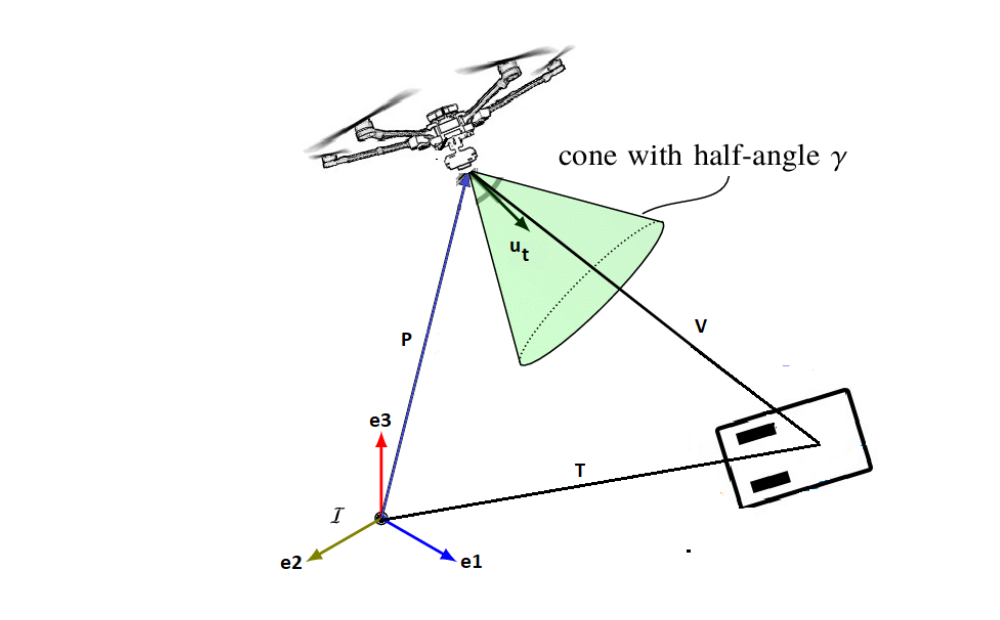
\includegraphics[width=0.85\columnwidth]{figures/thesis_fov_cone.png}
\caption{FOV cone geometry, reproduced from \cite{pinto_thesis} (its own half-angle label, $\gamma$, is this paper's $\alpha$). $s_{\text{fov}}\ge0$ exactly when the bearing to the target, $V$, sits inside the cone.}
\label{fig:fovcone}
\end{figure}

\emph{Issue:} squaring the raw hinge already makes it continuously differentiable at $s_{\text{fov}}=0$, but its second derivative still jumps from 0 to 2 there; since the solver's Gauss--Newton Hessian (Section~\ref{sec:arch}) depends on curvature, not just gradient, a shallow $\beta$ leaves this jump active near the operating point and causes command chatter: sharpening $\beta$ from 5 to 20 drops peak yaw jerk from 42.16 to 6.34~rad/s$^2$ and eliminates all 40 command sign changes (Appendix, Table~\ref{tab:beta}). Separately, this cost only keeps the target inside the cone; it does not pull it toward the center, which an added centering term, $r_{\text{center}} = 1-\cos\gamma$, was needed to fix once the tracking band (Section~\ref{sec:cost-track}) stopped doing so implicitly.

\subsection{Collision Avoidance}
\label{sec:cost-collision}

$d_{\text{safe}}$ sums the drone radius, one voxel width, and a staleness margin bounding how much the ESDF can change between linearizing it and acting on it, found empirically by logging the worst observed gap between a stale linearization and a fresh query (0.0649~m, rounded to 0.07~m):
\begin{equation}
d_{\text{safe}} = \underbrace{0.15}_{\text{radius}} + \underbrace{0.05}_{\text{voxel}} + \underbrace{0.07}_{\text{staleness}} = 0.27 \text{ m.}
\end{equation}
Collision avoidance enters \eqref{eq:mpc} as a slacked constraint, $d_{\text{lin}}(p) \ge d_{\text{safe}} - s$, penalized $z_l s + \tfrac12 Z_l s^2$.

\emph{Issue:} as a squared-hinge \emph{cost} (the initial formulation), $r_{\text{obs}}=\max(0,d_{\text{safe}}-d_{\text{lin}})$, the gradient $2W(d_{\text{safe}}-d_{\text{lin}})$ vanishes at the boundary, so no finite weight achieves exact clearance (Appendix, Table~\ref{tab:weightsweep}). Reformulating as a constraint fixes this: the slack's linear term has gradient $z_l$, a constant that does not vanish at $s=0$, the classical exact-penalty property a quadratic cost never has.

\subsection{Occlusion Cost}
\label{sec:cost-occ}

Occlusion is costed by linearizing the ESDF at a point along the drone-to-target sightline,
\begin{equation}
\text{occ}_{p_0}(s) = (1-s)\, p + s\, p_{\text{target}}, \qquad r_{\text{occ}} = \max(0,\, \tau - d(s)),
\label{eq:occpoint}
\end{equation}
with $d(s)$ the ESDF linearized at $\text{occ}_{p_0}(s)$ and $\tau$ an activation margin. Differentiating with respect to the drone's own position $p$,
\begin{equation}
\frac{\partial\, r_{\text{occ}}}{\partial p} = -(1-s)\,\nabla d.
\label{eq:chainrule}
\end{equation}

\begin{figure}[t]
\centering
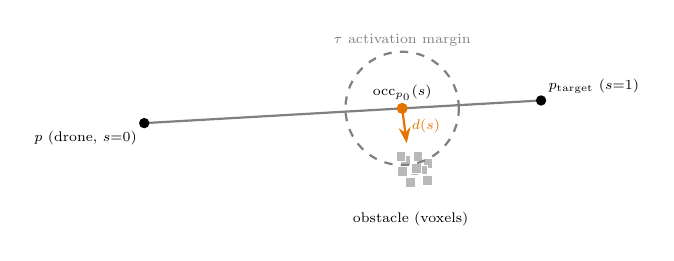
\begin{tikzpicture}[>={Stealth[length=2mm]}, thick, scale=0.72, every node/.style={transform shape}]
\coordinate (D) at (0,0);
\coordinate (T) at (7,0.4);
\coordinate (P0) at (4.55,0.26);
\coordinate (Obs) at (4.7,-0.9);
\draw[gray] (D) -- (T);
\filldraw[black] (D) circle (2pt) node[below left, font=\scriptsize] {$p$ (drone, $s{=}0$)};
\filldraw[black] (T) circle (2pt) node[above right, font=\scriptsize] {$p_{\text{target}}$ ($s{=}1$)};
\filldraw[orange!90!black] (P0) circle (2.2pt);
\node[above, font=\scriptsize] at (P0) {$\text{occ}_{p_0}(s)$};
\foreach \dx/\dy in {-0.18/0.16, 0.04/0.23, 0.22/0.11, -0.23/-0.04, -0.01/-0.02,
                     0.21/-0.19, -0.09/-0.23, 0.13/-0.01, -0.26/0.23, 0.02/0.02}{
  \filldraw[fill=gray!55, draw=white, line width=0.3pt] ($(Obs)+(\dx,\dy)$) rectangle ++(0.17,0.17);
}
\node[font=\scriptsize] at ($(Obs)+(0,-0.8)$) {obstacle (voxels)};
\draw[->, color=orange!90!black] (P0) -- ($(Obs)!0.55cm!(P0)$) node[midway, right, font=\scriptsize] {$d(s)$};
\draw[dashed, gray] (P0) circle (1.0);
\node[font=\scriptsize, gray] at ($(P0)+(0,1.2)$) {$\tau$ activation margin};
\end{tikzpicture}
\caption{Occlusion cost geometry. $\text{occ}_{p_0}(s)$ linearizes the ESDF at a point on the drone-to-target sightline; $r_{\text{occ}}$ activates once $d(s)<\tau$.}
\label{fig:occgeom}
\end{figure}

\emph{Issue:} this gradient vanishes structurally as $s\to1$ (obstruction near the target), independent of weight. Section~\ref{sec:occanalysis} derives why and tests two fixes, neither of which resolves it.

\subsection{Weights}
\label{sec:weights}

Table~\ref{tab:weights} summarizes the operating weights and their source. None were derived analytically; each was set by a sweep (Section~\ref{sec:cost-fov}, \ref{sec:cost-collision}, Appendix) or carried over unchanged once an earlier sweep had already validated it.

\begin{table}[t]
\centering
\caption{Operating weights and justification.}
\label{tab:weights}
\begin{tabular}{llp{3.6cm}}
\hline
Residual & Value & Source \\
\hline
$r_{\text{pos}}$ (Baseline) & 100 / 200 & stage/terminal, carried from initial tuning \\
$r_{\text{dist}}, r_{\text{elev}}, r_{\text{azimuth}}$ (Band) & $\approx$20--100 each & zero in Baseline rows, active only once $r_{\text{pos}}$ is zeroed \\
$r_{\text{fov}}$, $\beta$ & 100, 20 & $\beta$ swept (Table~\ref{tab:beta}) \\
$r_{\text{occ}}$, $\tau$ & 20, 1.68 m & $\tau$ = FOV width at target range \\
collision $z_l$, $Z_l$ & 10000, 100 & $z_l$ large for exact penalty \\
rate regularization & 15 & carried from initial tuning \\
\hline
\end{tabular}
\end{table}

\section{Occlusion Cost: Structural Analysis}
\label{sec:occanalysis}

\subsection{The Vanishing-Gradient Failure Mode}
\label{sec:occlusion-vanish}

In \eqref{eq:chainrule}, $(1-s)$ is the entire sensitivity of the occlusion cost to the drone's own position. As the real obstruction approaches the target end of the sightline, $s\to1$, this factor, and the gradient the drone feels, go to zero regardless of weight. This is exactly the case collision avoidance (Section~\ref{sec:cost-collision}), which only sees obstacles near the drone, cannot substitute for: the occlusion term is weakest exactly where it is the only term that could help.

Fig.~\ref{fig:esdf} shows this geometry on a real evaluation-suite run: the sightline runs from the drone to the target inside the camera frustum, with own\_map's occupied voxels standing in for the ESDF obstacle, occlusion cost off (left) and on (right), same tick.

\begin{figure*}[t]
\centering
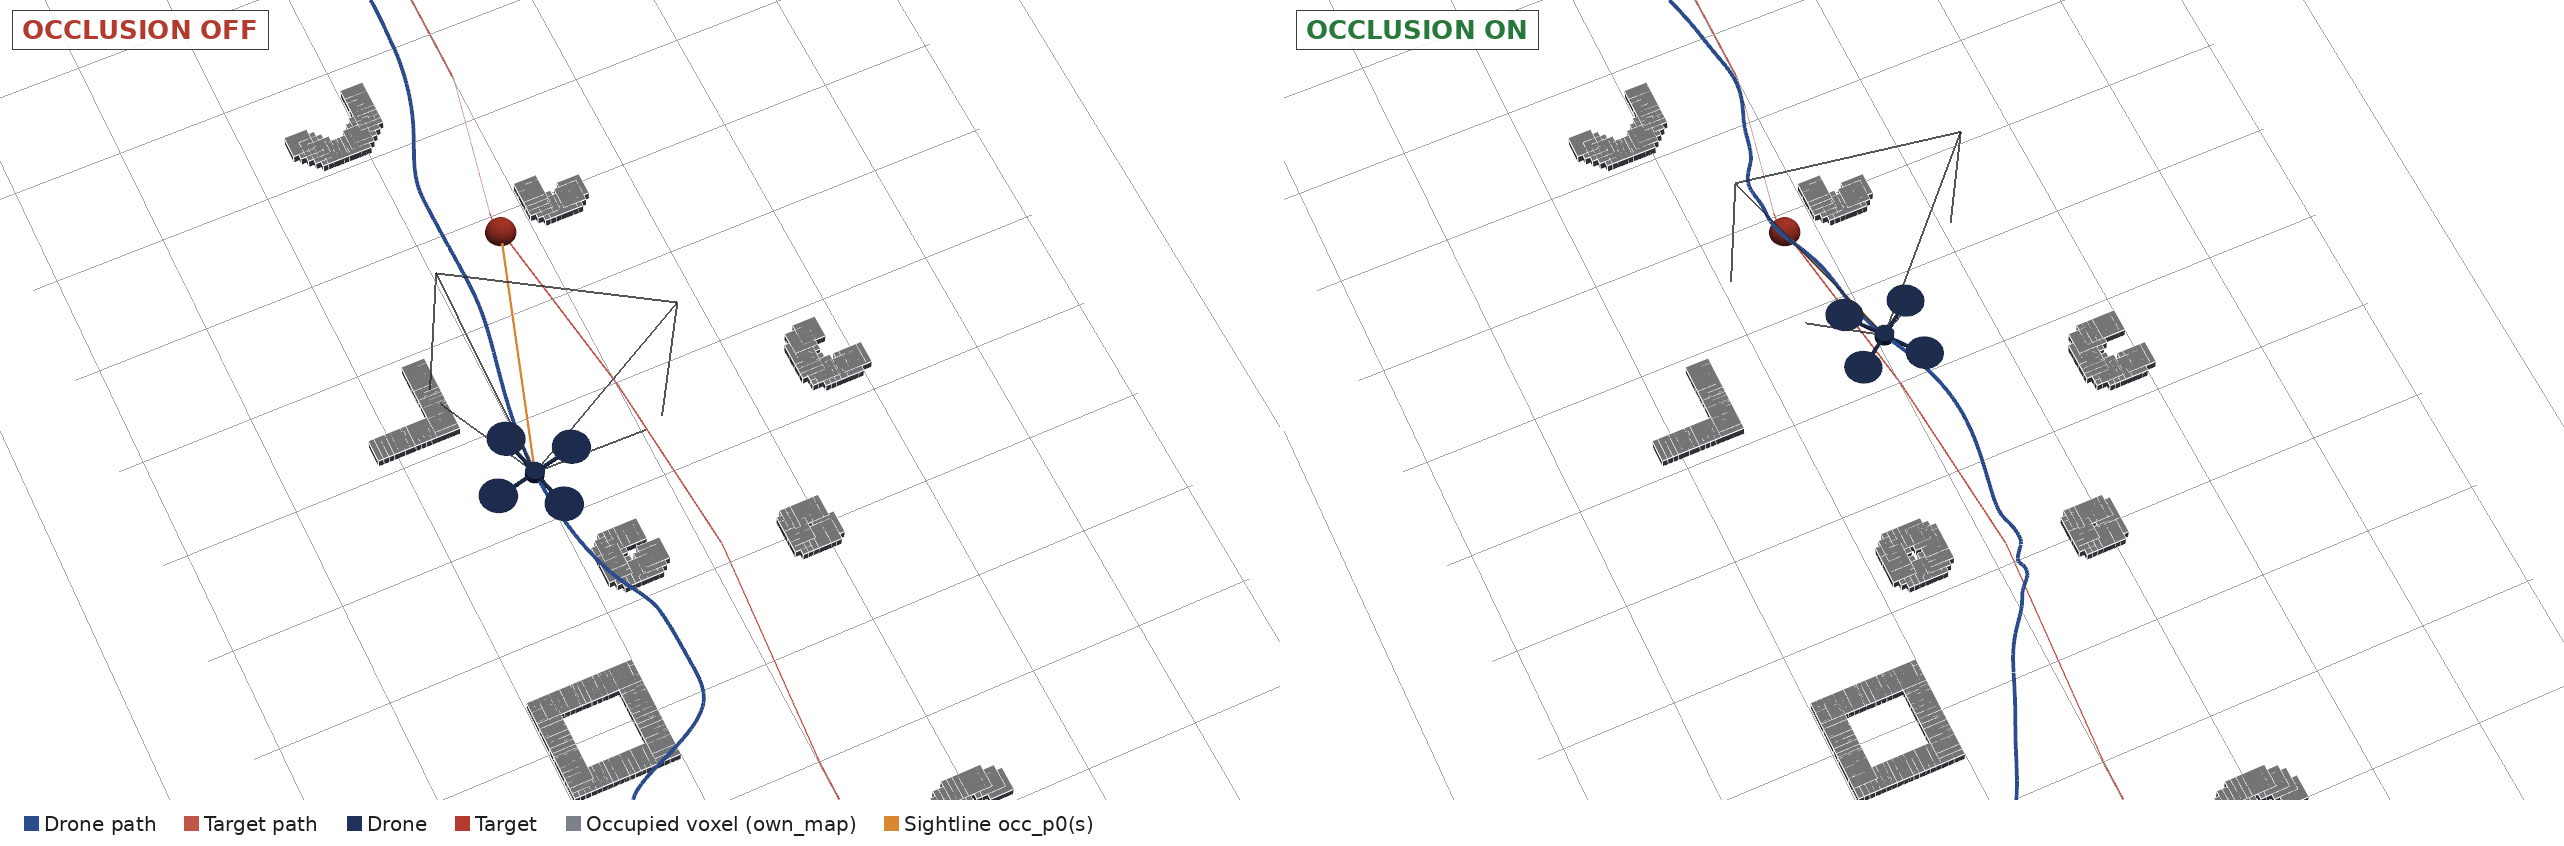
\includegraphics[width=\textwidth]{figures/esdf_sightline.png}
\caption{Third-person technical view, zoomed on the occluded region, occlusion cost off (left) and on (right), same scenario tick as Fig.~\ref{fig:footage}. own\_map's real occupied voxels (grey) are drawn in 3-D, not the ESDF's scalar field directly; the camera frustum, drone/target paths, and the sightline $\text{occ}_{p_0}(s)$ from \eqref{eq:occpoint} are overlaid.}
\label{fig:esdf}
\end{figure*}

\subsection{Candidate Fix: Hard-Min vs. Soft-Min Combination}
\label{sec:occlusion-hardsoft}

A natural fix costs several fixed sightline fractions instead of one adaptive point, so no sample's $(1-s)$ is itself a function of where the obstruction sits. The hard minimum, $d_{\min}(p)=\min_i d_i(p)$, is non-smooth where two samples tie, and the solver's Gauss--Newton Hessian jumps discretely across that tie, built only from whichever sample currently wins. A soft minimum,
\begin{equation}
d_{\text{soft}}(p) = -\frac{1}{\beta}\log \sum_i e^{-\beta d_i(p)},
\label{eq:softmin}
\end{equation}
blends all samples by softmax weight $w_i$, giving $\bar{g}=\sum_i w_i(1-s_i)\nabla d_i$, continuous everywhere, recovering the hard case as $\beta\to\infty$. Neither removes the underlying failure: if the obstruction genuinely sits near the target, whichever sample is nearest it still carries a small $(1-s)$ there.

Both were tested on the same scenario, varying only the combination rule (Appendix, Table~\ref{tab:hardsoft}): closest approach, field-of-view exceedance, and mean occlusion stayed within a narrow band of each other and of the adaptive single-point baseline. Only solver time moved consistently with $\beta$, rising with the curvature term \eqref{eq:softmin} adds near a tie, not with occlusion quality.

\subsection{Candidate Fix: A Steeper Penalty Function}
\label{sec:occlusion-steeper}

A second candidate reshapes the penalty, $r(d)=1/d-1/\tau$, an artificial-potential-field form growing faster as distance shrinks. This changes only the scalar multiplying the gradient direction; it has no effect on $(1-s)$. Multiplying zero by a steeper function of $d$ is still zero. It also reintroduces a singularity at $d=0$, the same class of problem as an unrelated earlier formula in this project whose derivative diverged at the system's own target operating point and caused a real collision (not detailed further, as it belongs to ongoing work).

\subsection{The Underlying Geometric Cause}

Neither candidate changes the parametrization. $\text{occ}_{p_0}(s)$ is a point on a segment between a moving end (the drone) and a fixed end (the target); a point near the fixed end barely moves when the moving end is perturbed, independent of sampling or aggregation. An obstacle occluding the sightline close to the target is, to first order, not something the drone's own position has leverage over.

\begin{figure}[t]
\centering
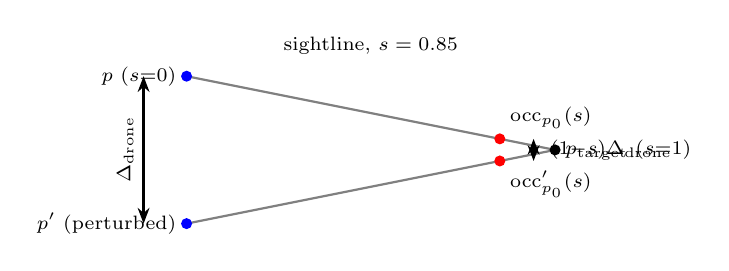
\begin{tikzpicture}[>={Stealth[length=2mm]}, thick, scale=0.78]
\coordinate (T) at (6,0);
\coordinate (D) at (0,1.2);
\coordinate (Dp) at (0,-1.2);
\coordinate (P) at (5.1,0.18);
\coordinate (Pp) at (5.1,-0.18);
\draw[gray] (D) -- (T);
\draw[gray] (Dp) -- (T);
\filldraw[black] (T) circle (2pt);
\node[right, font=\scriptsize] at (T) {$p_{\text{target}}$ ($s{=}1$)};
\filldraw[blue] (D) circle (2pt);
\node[left, font=\scriptsize] at (D) {$p$ ($s{=}0$)};
\filldraw[blue] (Dp) circle (2pt);
\node[left, font=\scriptsize] at (Dp) {$p'$ (perturbed)};
\filldraw[red] (P) circle (2pt);
\filldraw[red] (Pp) circle (2pt);
\node[above right, font=\scriptsize] at (P) {$\text{occ}_{p_0}(s)$};
\node[below right, font=\scriptsize] at (Pp) {$\text{occ}_{p_0}'(s)$};
\draw[<->] (-0.7,1.2) -- (-0.7,-1.2);
\node[rotate=90, font=\scriptsize] at (-1.0,0) {$\Delta_{\text{drone}}$};
\draw[<->] (5.65,0.18) -- (5.65,-0.18);
\node[right, font=\scriptsize] at (5.75,0) {$(1{-}s)\Delta_{\text{drone}}$};
\node[font=\scriptsize] at (3,1.7) {sightline, $s=0.85$};
\end{tikzpicture}
\caption{The lever-arm geometry behind \eqref{eq:chainrule}. Perturbing the drone from $p$ to $p'$ by $\Delta_{\text{drone}}$ moves the linearization point $\text{occ}_{p_0}(s)$ by only $(1-s)\Delta_{\text{drone}}$. At $s=0.85$, shown here, the point moves at 15\% of the drone's own displacement; as $s\to1$ this ratio, and the gradient in \eqref{eq:chainrule}, goes to zero.}
\label{fig:leverarm}
\end{figure}

Fig.~\ref{fig:leverarm} makes this concrete: the same perturbation $\Delta_{\text{drone}}$ produces a far smaller displacement of the linearization point once $s$ is close to 1, by exactly the factor $(1-s)$ already derived algebraically in \eqref{eq:chainrule}. No choice of sample fraction, combination rule, or penalty shape changes this ratio, since it is a property of where the point sits on the segment, not of what is evaluated there.

\subsection{Implication for a Working Formulation}
\label{sec:occlusion-implication}

What retains sensitivity near the target is the sightline's angle, not a point's position on it: moving the drone swings the sightline's bearing substantially even when the obstruction sits near the target, the same lever-arm effect that makes a point there barely move. This points to an angular or frustum-volume formulation, not a reparametrization of the same point-on-segment idea. It is not built here; Section~\ref{sec:future} states it as the next step.

\section{Results}
\label{sec:results}

\begin{table*}[t]
\centering
\caption{Measured on the \texttt{forest\_clutter} evaluation scenario. Reacq. counts lost-contact events (leaving the FOV cone or exceeding 90\% occlusion).}
\label{tab:results}
\begin{tabular}{lcccc}
\hline
Configuration & Clearance (m) & Rate max (deg/s) & Occlusion mean/max (\%) & Reacq. \\
\hline
Baseline (fixed tracking, occlusion off) & 0.30 & 127.9 & 63.8 / 84.8 & 0 \\
Baseline, occlusion cost on & 0.35 & 86.4 & 62.6 / 82.1 & 1 \\
Band follower, occlusion on & 0.40 & 60.0 & 63.2 / 100.0 & 4 \\
Band follower + centering term & 0.38 & 61.8 & 65.8 / 100.0 & 1 \\
\hline
\end{tabular}
\end{table*}

Table~\ref{tab:results} summarizes the configurations introduced in Sections~\ref{sec:cost-track}--\ref{sec:cost-occ}. The scenario's obstacle layout and target trajectory are deterministic, so each row is a single run of its configuration, not an average over repeats; the numbers below should be read as one realization each, not as means with an implied variance. Turning the occlusion cost on alone barely moves mean occlusion (63.8\% to 62.6\%), consistent with Section~\ref{sec:occlusion-vanish}: it only has real effect while the obstruction sits closer to the drone than to the target, and the gap is small enough on a single run that it should be treated as indicative, not conclusive, without repeated trials.

The band follower's reacquisition count (4 events, against 0 for the baseline) is the table's largest regression, and it traces directly to Section~\ref{sec:cost-track}: the Baseline pins $(x,y,z)$ to the trailer point, so framing is fixed by construction, while the Band follower opens a dead zone on distance, elevation, and azimuth to buy the clearance gain above, and nothing then re-centers the target once the drone uses that freedom to dodge an obstacle, since the field-of-view cost (Section~\ref{sec:cost-fov}) only penalizes leaving the cone, not drifting toward its edge. The centering term, $r_{\text{center}}=1-\cos\gamma$, recovers most of this (4 to 1) by rewarding boresight alignment directly, but not all of it: it does nothing for the occlusion cost's own weakness (Section~\ref{sec:occlusion-vanish}), and the lost-contact metric counts both failure modes as one event.

\begin{figure*}[t]
\centering
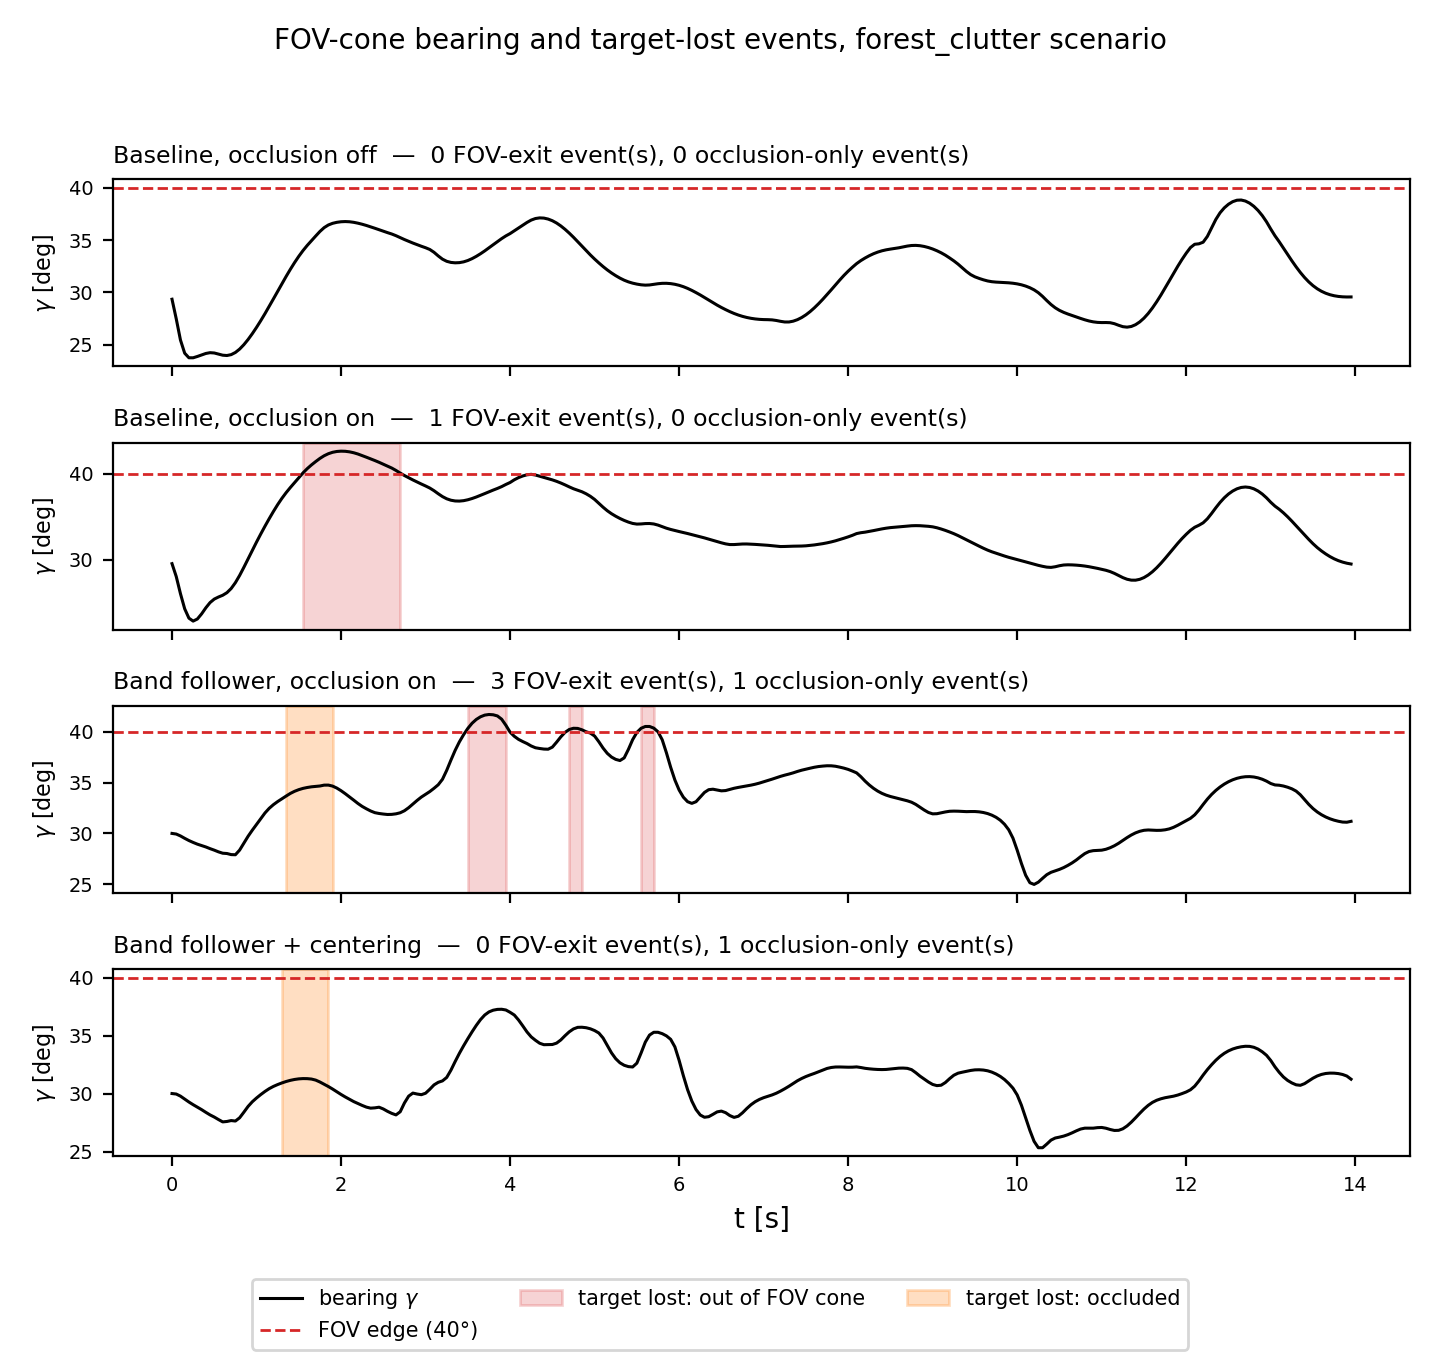
\includegraphics[width=\textwidth]{figures/fov_results.png}
\caption{Combined bearing angle $\gamma$ against the FOV half-angle threshold, for each row of Table~\ref{tab:results}, with Table~\ref{tab:results}'s merged Reacq.\ count split into its two causes: out of the FOV cone (red) vs.\ occluded past the lost-contact threshold (orange).}
\label{fig:fovresults}
\end{figure*}

Fig.~\ref{fig:fovresults} splits that merged count open. The Baseline's occlusion-off row never exceeds the cone; turning its occlusion cost on introduces one brief FOV excursion, not an occlusion-caused loss, at $t\approx2$~s. The Band follower's four events are three FOV-cone exits plus one occlusion loss, confirming the mechanism above: the centering term's fix (4 to 1) is visible directly as the three red spans disappearing from the bottom panel, with the one orange occlusion span -- the failure mode centering does not touch -- left unchanged.

\begin{figure*}[t]
\centering
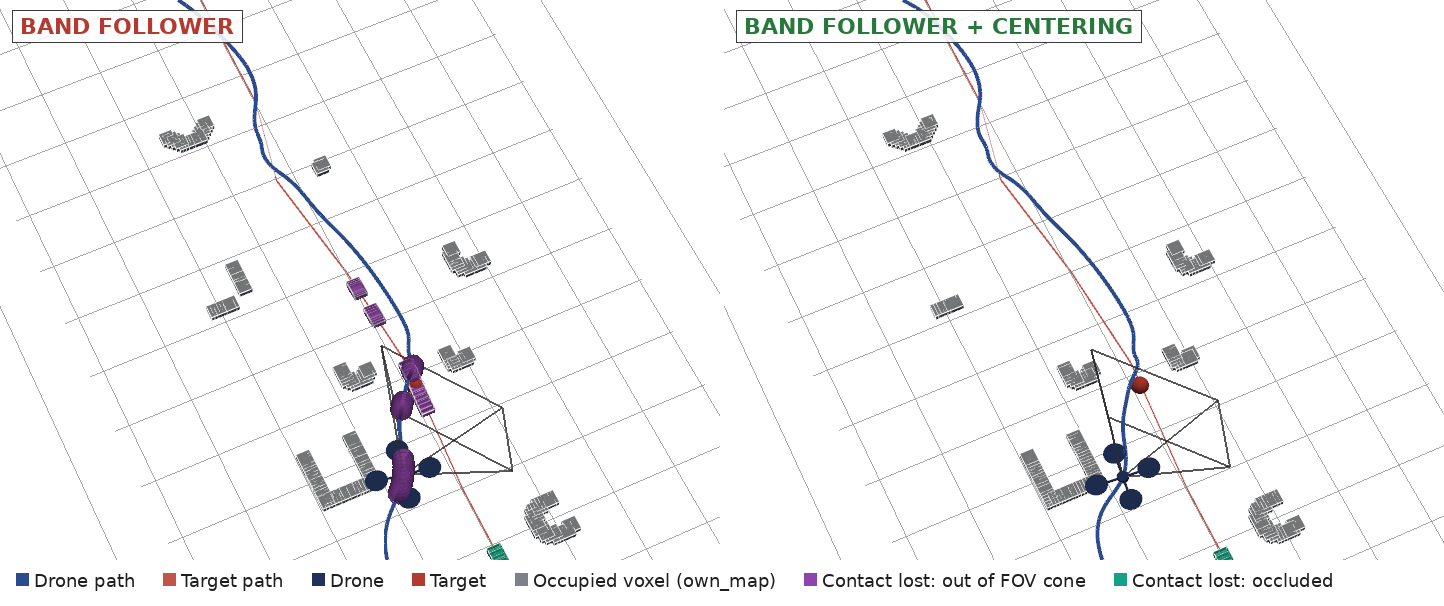
\includegraphics[width=\textwidth]{figures/fov_event_comparison.png}
\caption{Same tick ($t=3.75$~s) and scenario, Band follower (left) vs.\ Band follower + centering (right) -- the first of the three FOV-cone-exit events Fig.~\ref{fig:fovresults} shows disappearing. The target marker sits outside the frustum wireframe on the left, inside it on the right; the red path markers are the out-of-FOV mask drawn on the drone's position throughout the run, not just at this tick.}
\label{fig:fovevent}
\end{figure*}

Fig.~\ref{fig:fovevent} shows one of those three events directly: the same scenario tick, the Band follower's target has drifted past the cone edge while the centering variant, at that same instant, has already pulled it back inside.

No row resolves Section~\ref{sec:occanalysis}'s structural problem; each trades a different combination of its symptoms.

\begin{figure*}[t]
\centering
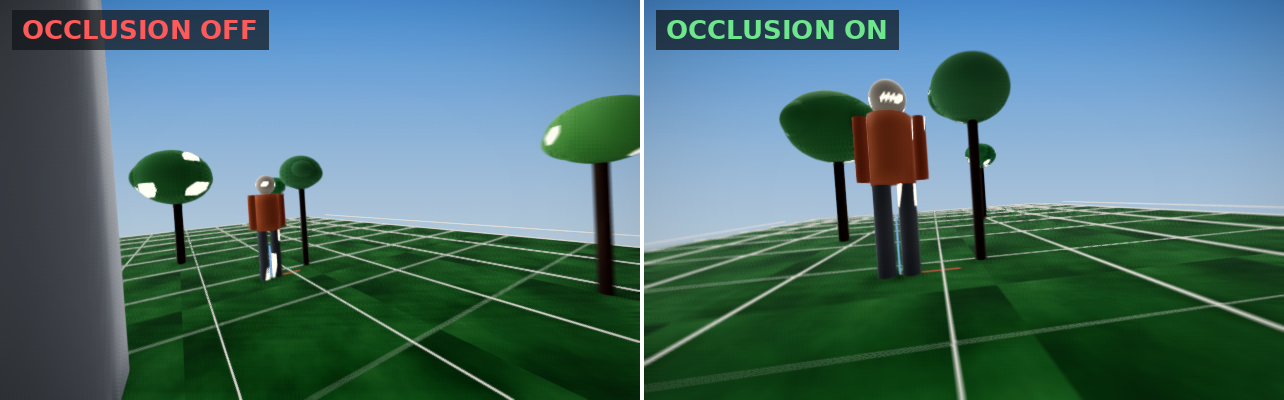
\includegraphics[width=\textwidth]{figures/footage_comparison.png}
\caption{Rendered onboard camera view, occlusion cost off (left) and on (right), same tick as Fig.~\ref{fig:esdf}.}
\label{fig:footage}
\end{figure*}

Fig.~\ref{fig:footage} shows the rendered view at the same tick as Fig.~\ref{fig:esdf}: obstacle clearance rises from 0.67~m (off) to 1.47~m (on), the same effect Table~\ref{tab:results} reports numerically, without the target leaving the frame in either case at this tick.

\section{Limitations and Future Work}
\label{sec:future}

\subsection{Toward an Angular/Frustum Formulation}
\label{sec:future-angular}

The direction in Section~\ref{sec:occlusion-implication}, costing angular sensitivity or an approximate frustum-obstacle intersection instead of a linearized point, is not implemented here. It is scoped as the next step: a closed-form cost and gradient well-conditioned under the one-step SQP\_RTI solver of Section~\ref{sec:arch}, tested against the scenario used throughout Sections~\ref{sec:occanalysis}--\ref{sec:results}.

\subsection{Remaining Approximation}

Even a working angular or frustum formulation would still rely on a local point-or-sphere approximation of the obstacle's surface, from the ESDF's value and gradient at one query location, not a true volumetric intersection. That would require the live occupancy grid inside the differentiable symbolic model the solver is generated from, unavailable at code-generation time in this architecture; an acknowledged limitation of the direction above, not a problem it is expected to resolve.

A related tuning result is worth recording here since it generalizes beyond this one residual: pinning the elevation residual $r_{\text{elev}}$ with a nonzero weight bought a narrower altitude band only by raising vertical acceleration, not lowering it, across the evaluation suite, so a tighter constraint was not a smoother one.

\subsection{Evaluation Scope}

Every comparison in Section~\ref{sec:results} and the Appendix is internal: configurations of this same controller against each other, on logged scenarios with no repeated trials (Section~\ref{sec:results}). There is no comparison against an external tracking method -- a potential-field or sampling-based planner, or a learned policy -- so the numbers here establish what the occlusion cost changes relative to this architecture's own baseline, not where this architecture sits relative to the field.

\section{Conclusion}

This paper reported three extensions to a perception-aware MPC for aerial target tracking: porting it from Python to C++ with a real-time ESDF replacing known obstacle shapes, moving collision avoidance from a cost to a slacked constraint, and introducing an occlusion-aware cost. The first two are measured improvements (Sections~\ref{sec:cost-collision}, \ref{sec:results}). The occlusion cost, in its point-linearized form, remains ineffective whenever the obstruction sits near the target rather than the drone, regardless of weight or sightline sampling. Two independent fixes were tested against this failure and both left it unchanged; the cause traces to the geometry of the point-on-segment parametrization itself, not to either candidate's own shortcomings. An angular or frustum-based reformulation, outlined in Section~\ref{sec:future}, has not yet been implemented or tested.

\appendix

\begin{table}[t]
\centering
\caption{Collision cost weight sweep, $d_{\text{safe}}=0.27$ m (Section~\ref{sec:cost-collision}).}
\label{tab:weightsweep}
\begin{tabular}{cc}
\hline
Weight & Closest approach (m) \\
\hline
10 & 0.00 \\
50 & 0.05 \\
100 & 0.10 \\
200 & 0.15 \\
500 & 0.20 \\
\hline
\end{tabular}
\end{table}

\begin{table}[t]
\centering
\caption{FOV softplus $\beta$ sweep, yaw-correction scenario (Section~\ref{sec:cost-fov}).}
\label{tab:beta}
\begin{tabular}{cccc}
\hline
$\beta$ & FOV exceed. (s) & Peak yaw jerk (rad/s$^2$) & Sign changes \\
\hline
5  & 0.30 & 42.16 & 40 \\
20 & 0.30 & 6.34  & 0  \\
\hline
\end{tabular}
\end{table}

\begin{table}[t]
\centering
\caption{Occlusion combination rule comparison (Section~\ref{sec:occlusion-hardsoft}).}
\label{tab:hardsoft}
\begin{tabular}{lccc}
\hline
Rule & Clearance (m) & Occl. mean (\%) & Solve time max (ms) \\
\hline
Adaptive (baseline) & 0.35 & 62.6 & -- \\
Hard-min & 0.30 & 63.3 & 2.98 \\
Soft-min, $\beta=1$ & 0.30 & 63.0 & 2.75 \\
Soft-min, $\beta=5$ & 0.30 & 63.3 & 4.60 \\
Soft-min, $\beta=20$ & 0.30 & 63.3 & 5.30 \\
\hline
\end{tabular}
\end{table}

\subsection{Evaluation Tooling}
\label{sec:appendix-tooling}

Two tools produced the numbers and tables above. A per-run metrics dashboard (Fig.~\ref{fig:dashboard}) plots clearance, occlusion, bearing offset, tracking error, solver timing, and body-rate smoothness against time for one run, with a pass/fail summary against this run's own thresholds at the bottom; Fig.~\ref{fig:timing} isolates one of its panels, the real-time budget claimed in Section~\ref{sec:arch}, directly: solve time, ESDF build time, and their sum against the 50~ms deadline, over the same run. A 16-scenario evaluation suite (hand-authored obstacle layouts and target motion profiles, not procedurally generated) runs every configuration change through a common gate set; Fig.~\ref{fig:contactsheet} is one suite overview grid, a top-down path thumbnail per scenario with a green or red border marking its gate result.

\begin{figure}[t]
\centering
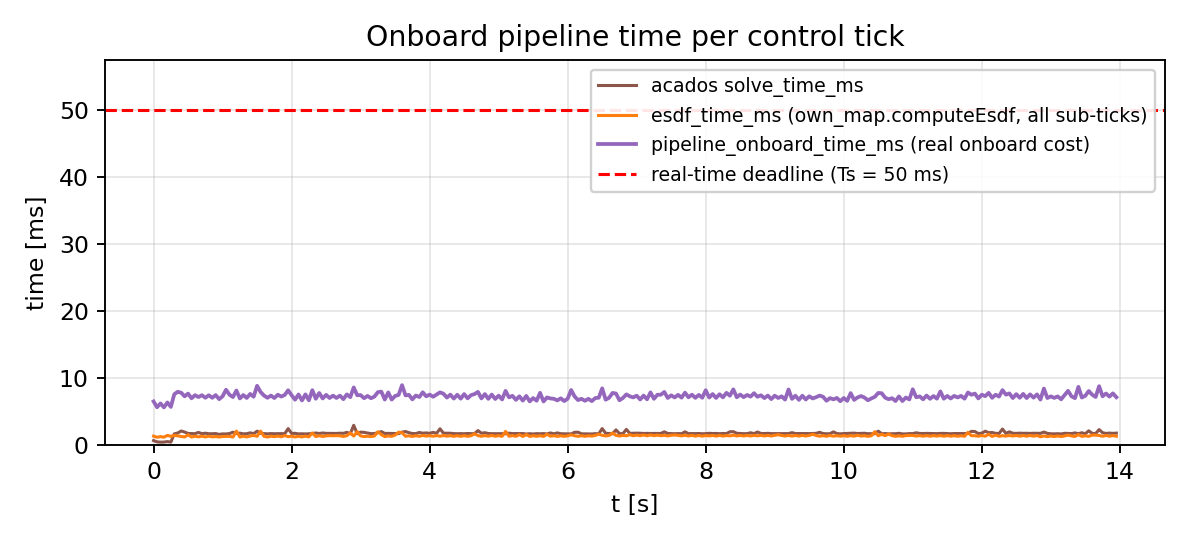
\includegraphics[width=\columnwidth]{figures/timing_breakdown.png}
\caption{Onboard pipeline time per control tick, same run as Fig.~\ref{fig:dashboard}. The solver (acados) and the ESDF rebuild together stay under 9~ms, well inside the 50~ms control-tick deadline (Section~\ref{sec:arch}).}
\label{fig:timing}
\end{figure}

\begin{figure*}[p]
\centering
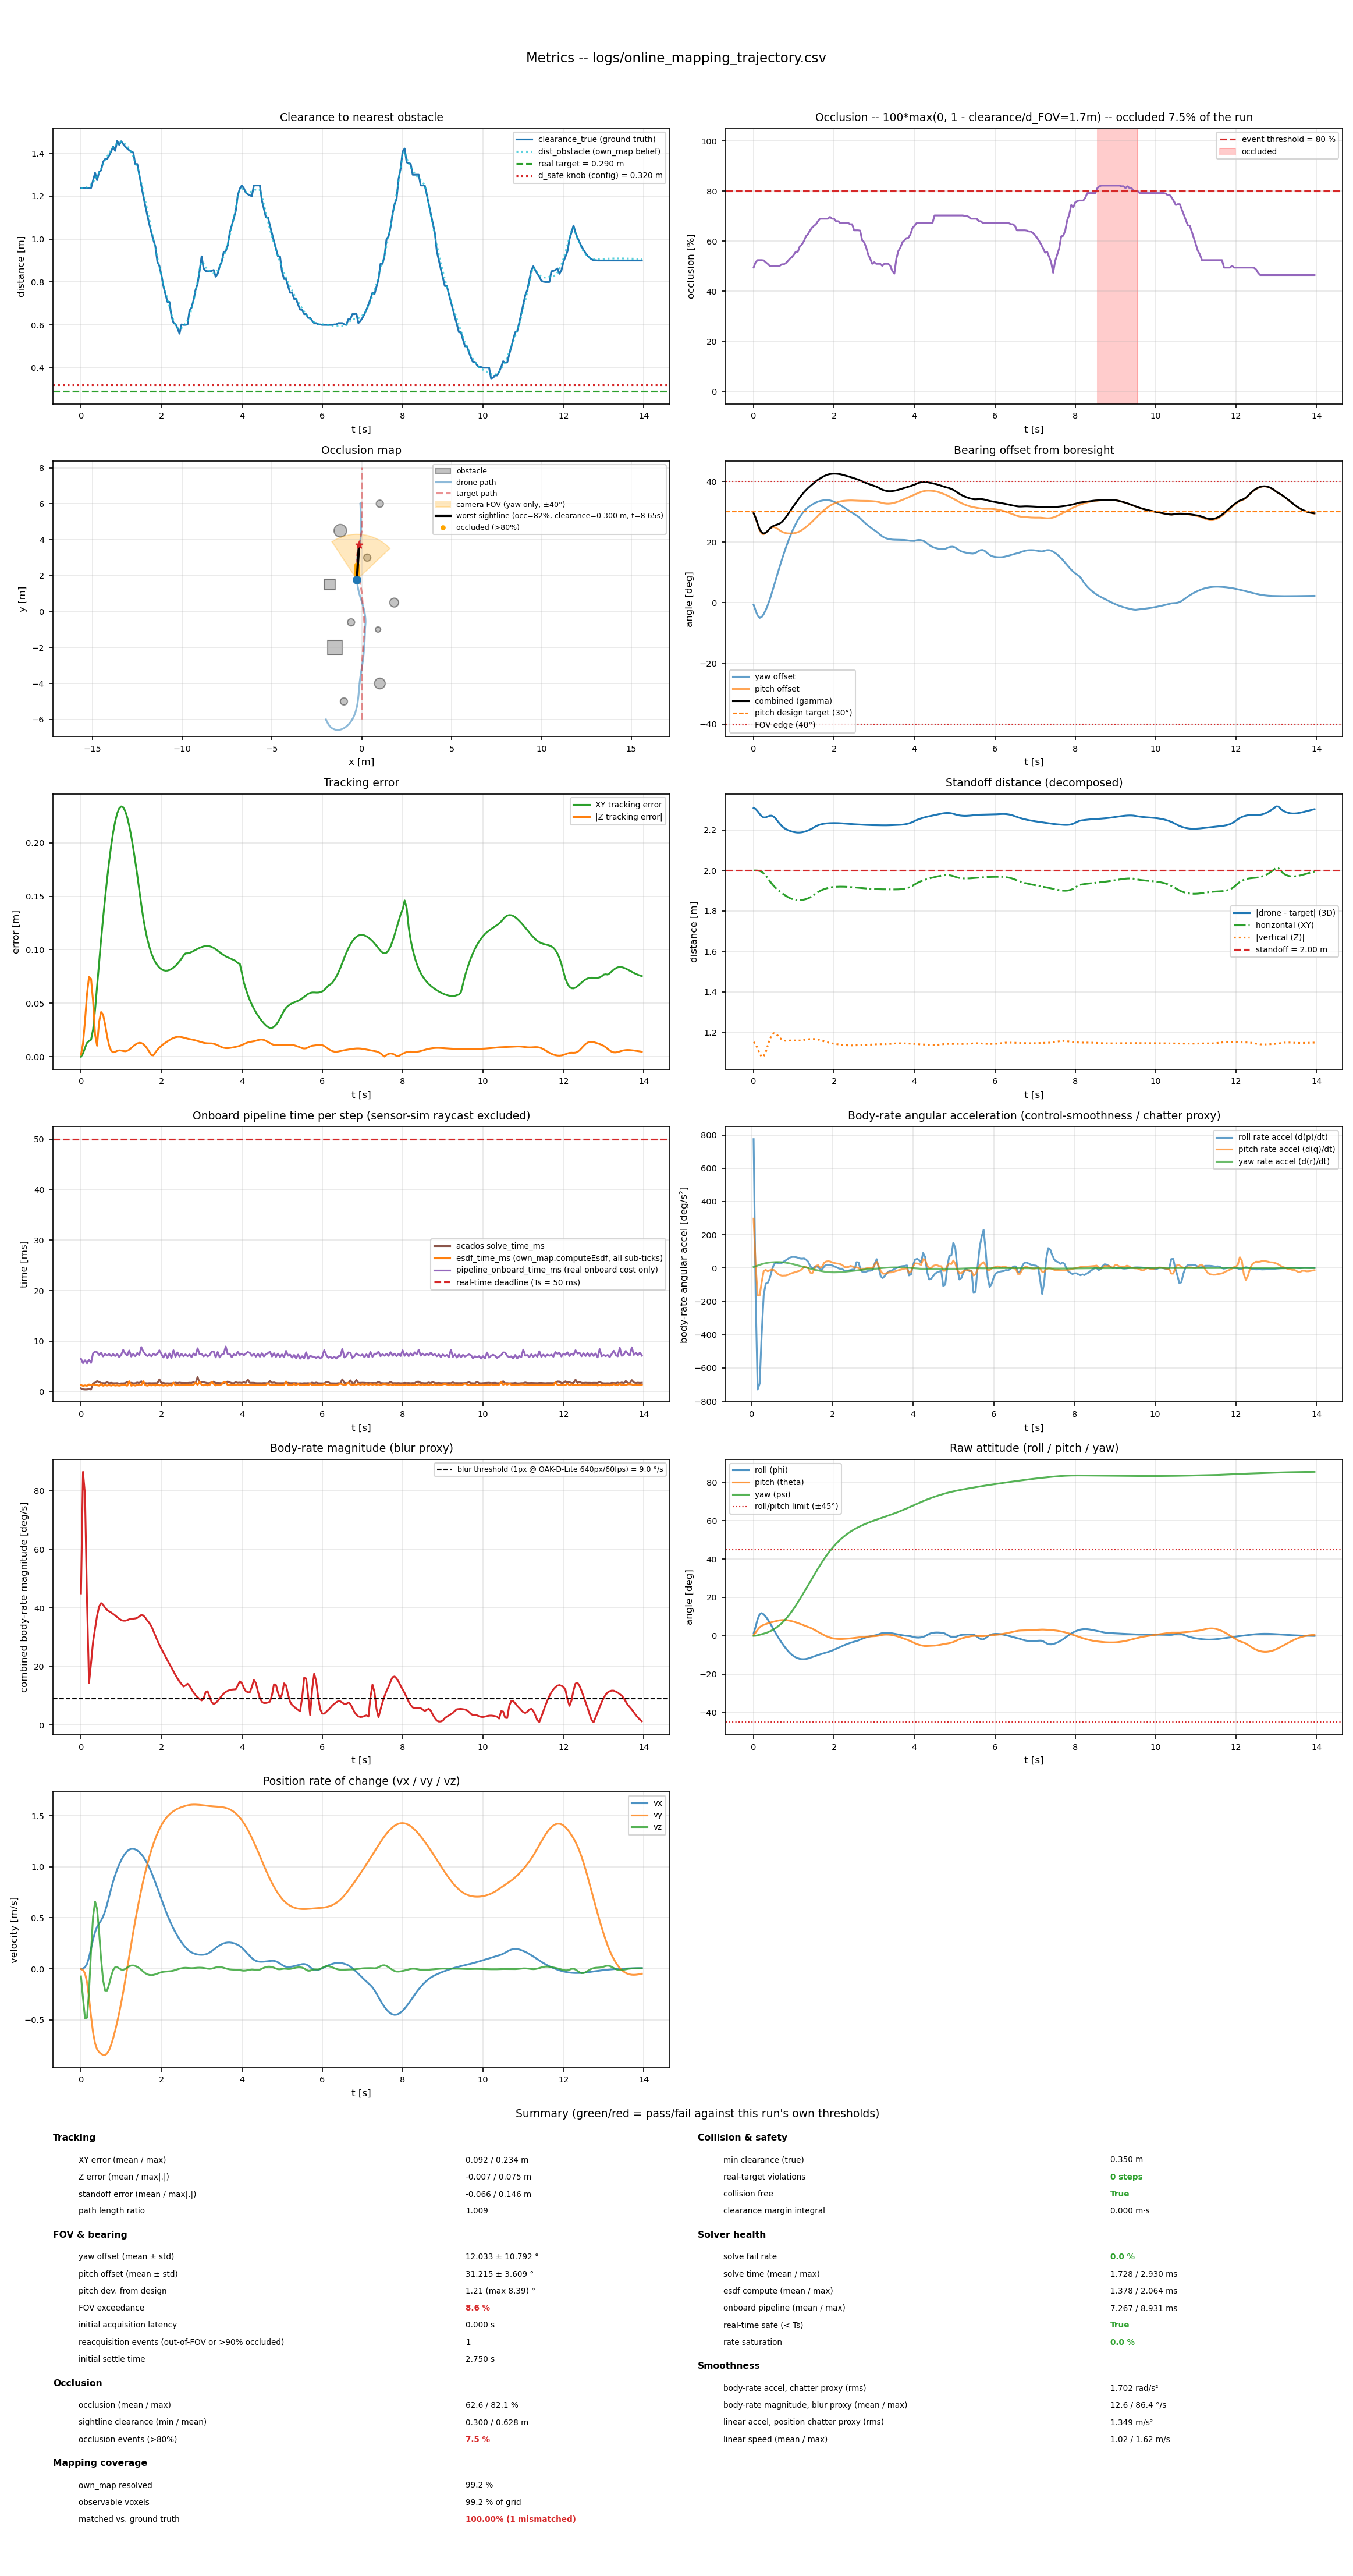
\includegraphics[width=0.85\textwidth]{figures/metrics_dashboard.png}
\caption{Per-run metrics dashboard, generated from one logged trajectory. Twelve panels covering clearance, occlusion, bearing, tracking error, solver and pipeline timing, and smoothness, with a numeric pass/fail summary below.}
\label{fig:dashboard}
\end{figure*}

\begin{figure*}[p]
\centering
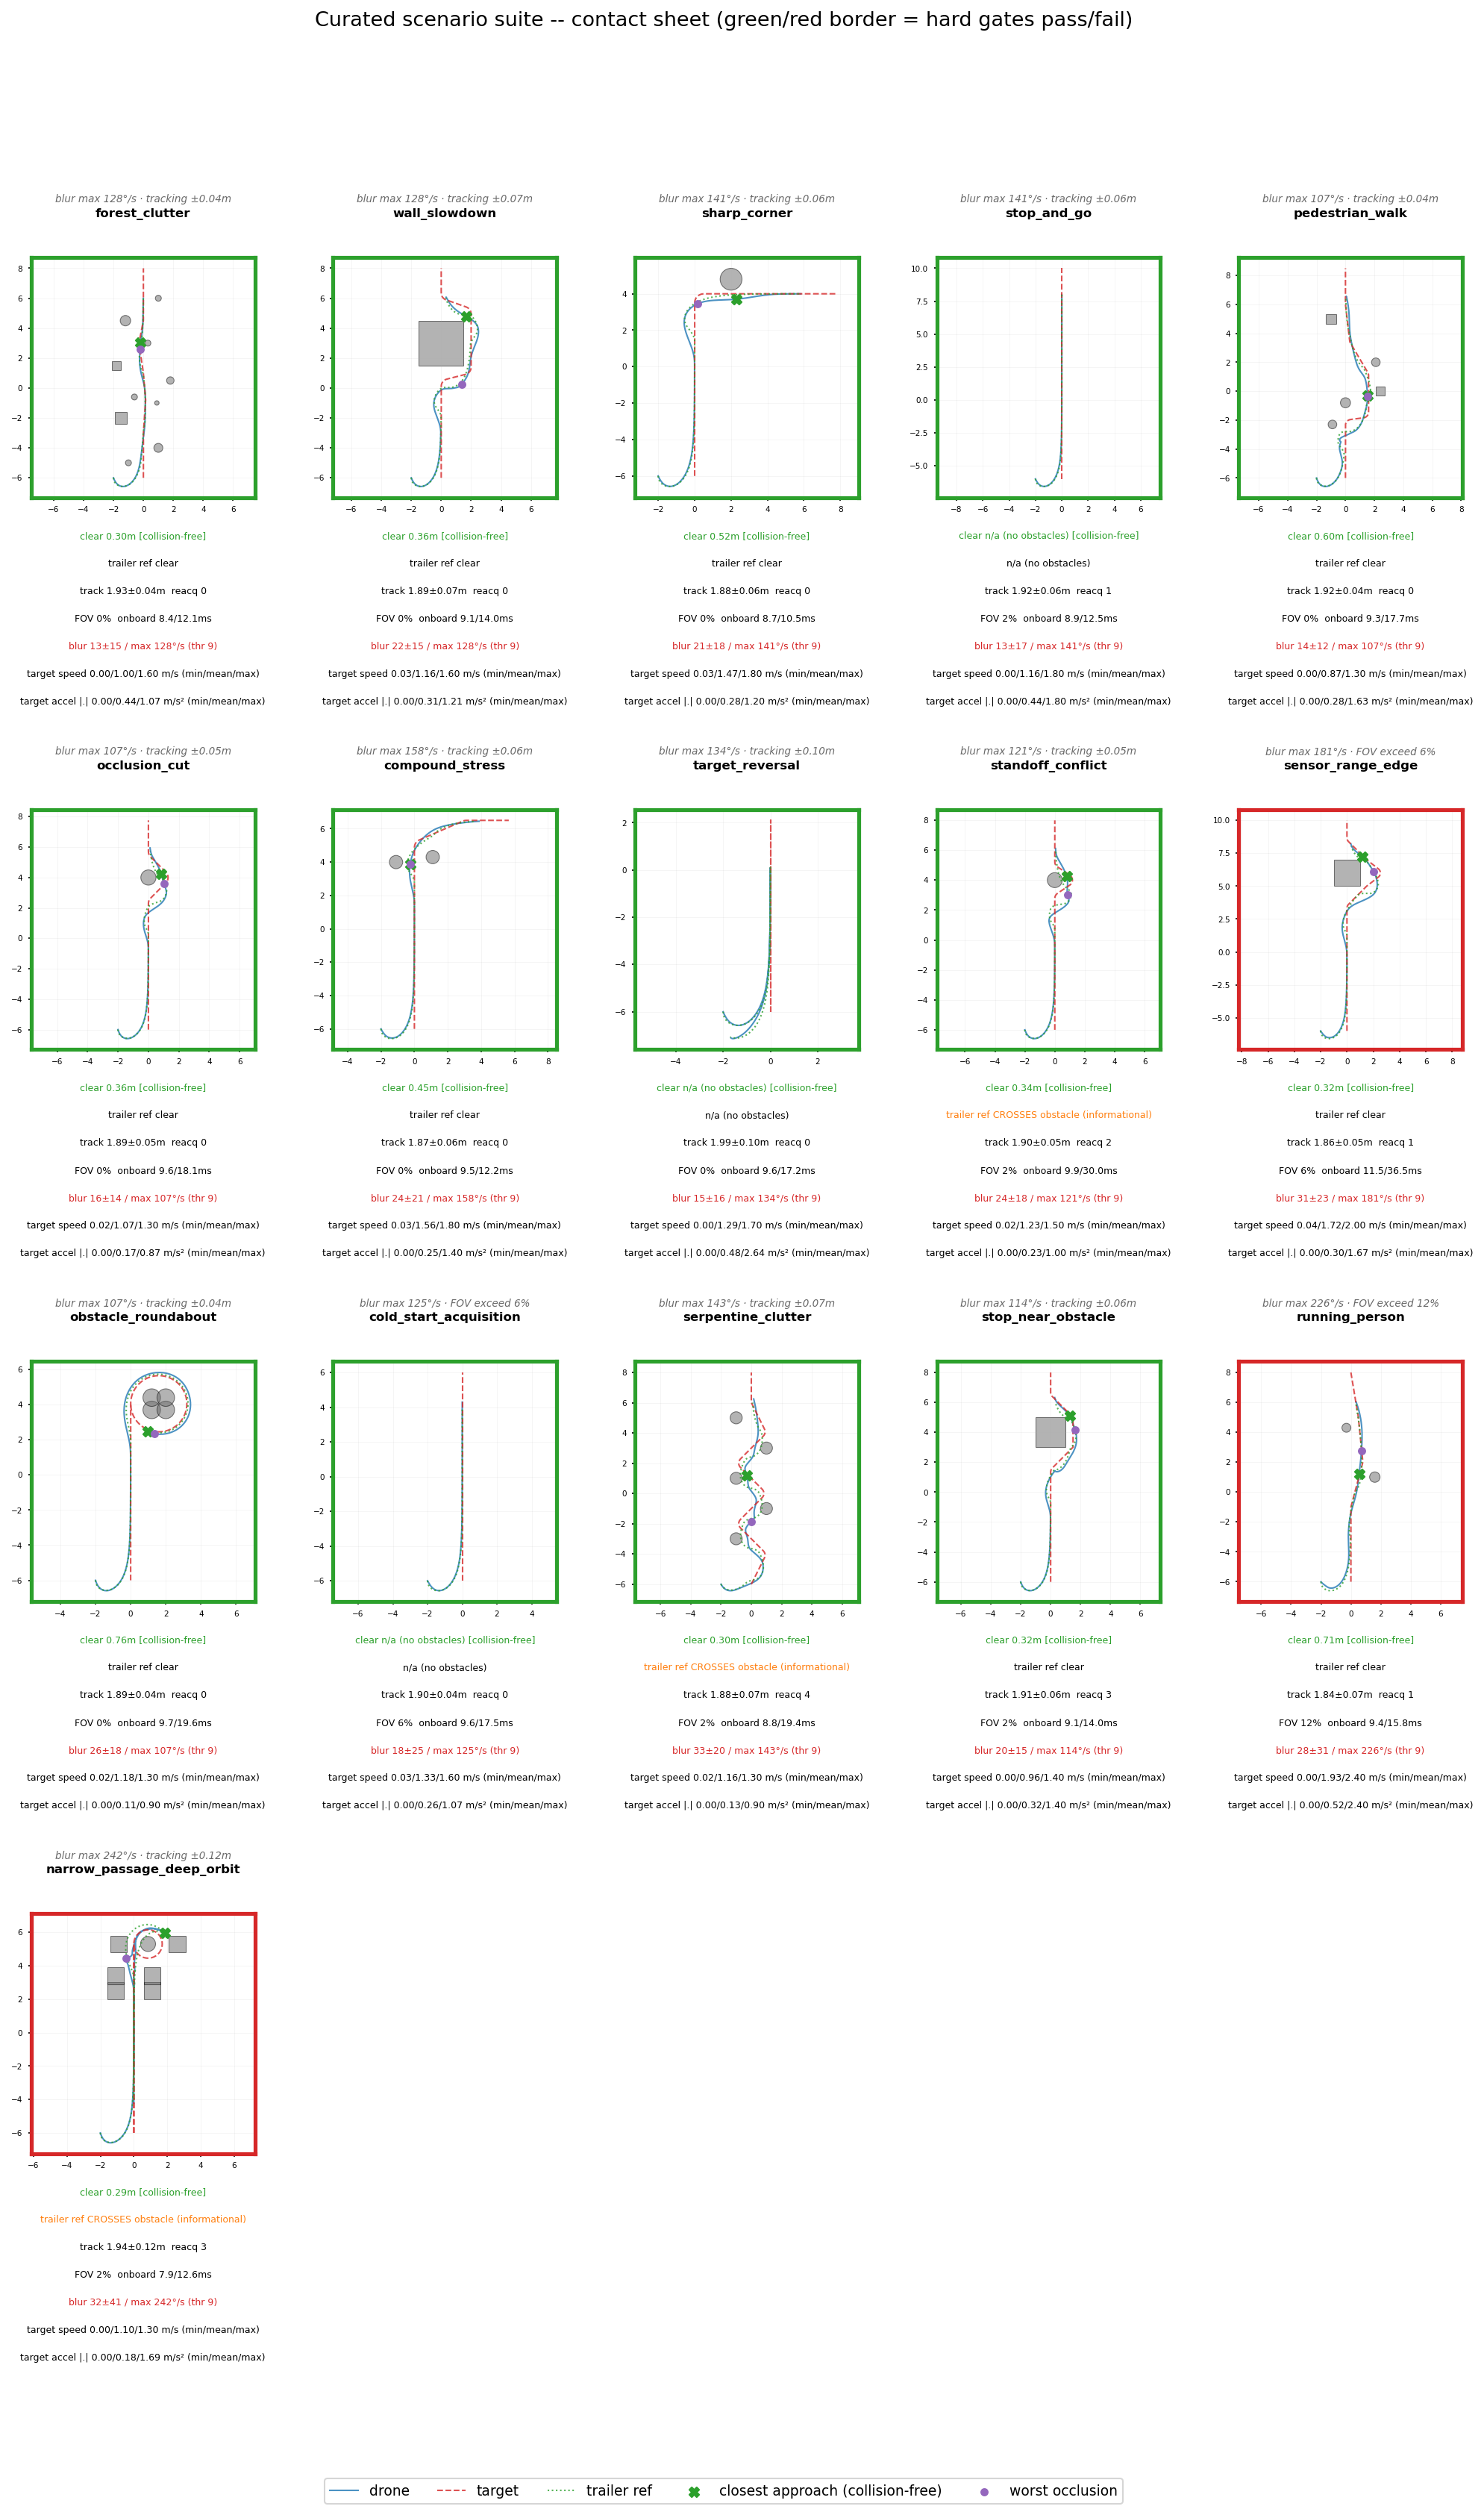
\includegraphics[width=0.85\textwidth]{figures/scenario_contact_sheet.png}
\caption{Suite overview grid across the 16-scenario evaluation suite. Each panel is one scenario's top-down path; the border reports that scenario's own hard-gate result.}
\label{fig:contactsheet}
\end{figure*}

\bibliographystyle{IEEEtran}
\bibliography{references}

\end{document}
